%!TEX root = main.tex

\section{Experiments: Optimal Uber driver strategy}
\label{sec:experiments}

We consider the problem of evaluating optimal in expectation strategies for drivers using the on-demand ride service -- Uber. The driver strategies on this platform must be estimated from past data. This makes it a particularly attractive application for evaluating our framework.

\subsection{Data}
\label{sec:data}
% \todo[Harshal]{Fill in data gathering and how we used NYC taxi dataset to create representative Uber data}
To evaluate our methods, we need a representative sample of taxi rides data. To obtain this data, we strategically sample rides from the publicly available NYC taxi rides dataset and recreate them on the Uber platform using Uber API queries.

\spara{The Uber API}: 
The HTTP-based Uber API allows third-party developers to retrieve information about Uber. For our study, the most relevant endpoint of the API is \texttt{estimates/price}. It takes longitude and latitude of pick-up and drop-off locations and returns price estimates for all types of Uber products - UberX, UberXL and UberBlack. Along with the price estimates, it also provides the active surge multiplier rate at the pick-up location at the time of query. For the purpose of this study, we only focus on UberX, the most popular Uber product. We also use the \texttt{/products} endpoint to get information regarding the base fare, minimum fare, cost per minute and cost per unit distance for UberX. However, none of the Uber API endpoints provide information about the supply of UberX drivers or demand of passengers. To overcome this obstacle, we leverage the NYC taxi rides dataset.

\spara{NYC Taxi Rides Dataset}:
NYC taxi rides dataset\footnote{\url{http://www.nyc.gov/html/tlc/html/about/trip_record_data.shtml}} for the year 2015 contains yellow street-hail taxi records with fields capturing pick-up and drop-off dates/times, location co-ordinates, trip distances and fares. Each taxi record is accompanied with taxi location ID for the pick-up and drop-off locations. We use these location IDs to divide the city into a set of 29 non-overlapping zones.

\spara{Collecting Representative Data}:
To create a representative sample of data, our strategy relies on `recreating' NYC taxi rides virtually on the Uber platform. We use the price estimates endpoint to query rides from exact same pick-up to drop-off locations at exact same time of the day on same calendar date, but exactly one year later i.e, a real recorded ride from 2015 is virtually recreated in 2016. However, Uber imposes a rate limit of 1,000 API requests per hour per account. To respect these API limits, we randomly sample rides from every zone to every other zone in the city every 15 minutes. We assume that price estimates, travel times and distance of preferred travel paths by drivers do not vary significantly in 15 minutes. Chen {\etal}~\cite{chen2015peeking} have observed that 90\% of the surges on Uber platform have durations as multiples of 5 minutes. Hence, every 5 minutes, we also query the surge multiplier active within each zone.

Although the \texttt{estimates/time} endpoint of the Uber API returns the estimated waiting time for a passenger at a particular location, it provides no information on the supply of UberX cars in the neighborhood of a location. Consequently, we do not possess an exact estimate of the time spent by an Uber driver waiting for a passenger in a particular zone. However, in the next section, we provide a methodology to compute a conservative estimate of the driver waiting time in a particular zone at any time of the day using the successful passenger pick-up information from the NYC taxi rides dataset.

Using our methodology, we collected data for a period of 6 months, recreating rides from October, 2015 till March, 2016. However, due to the periodicity of the data, we provide experimental results for one week starting October 18, 2015\footnote{Our results do not vary qualitatively across different weeks.}.

\subsection{Experimental Setup}
In this section, we describe how we used the data collected in the previous section for modeling the dynamics of the city and an individual driver as described in Section \ref{sec:problem_setup}.


\spara{Modeling city}:
We divide each 24-hour day of the week in 144 time-slices of duration 10 minutes each, indexed by their start time. While modeling the city, the $c(i,j)$ entry of the count matrix $\countmatrix^t$ is the total number of rides from zone $i$ to zone $j$ in a 30 minute long time window centered around the time-slice $t$.  For example, Figure \ref{fig:demand_heatmap} plots the count matrix {\countmatrix} at different times of the day showing the variation in the total number of rides starting from each zone.

\begin{figure}
	\centering
	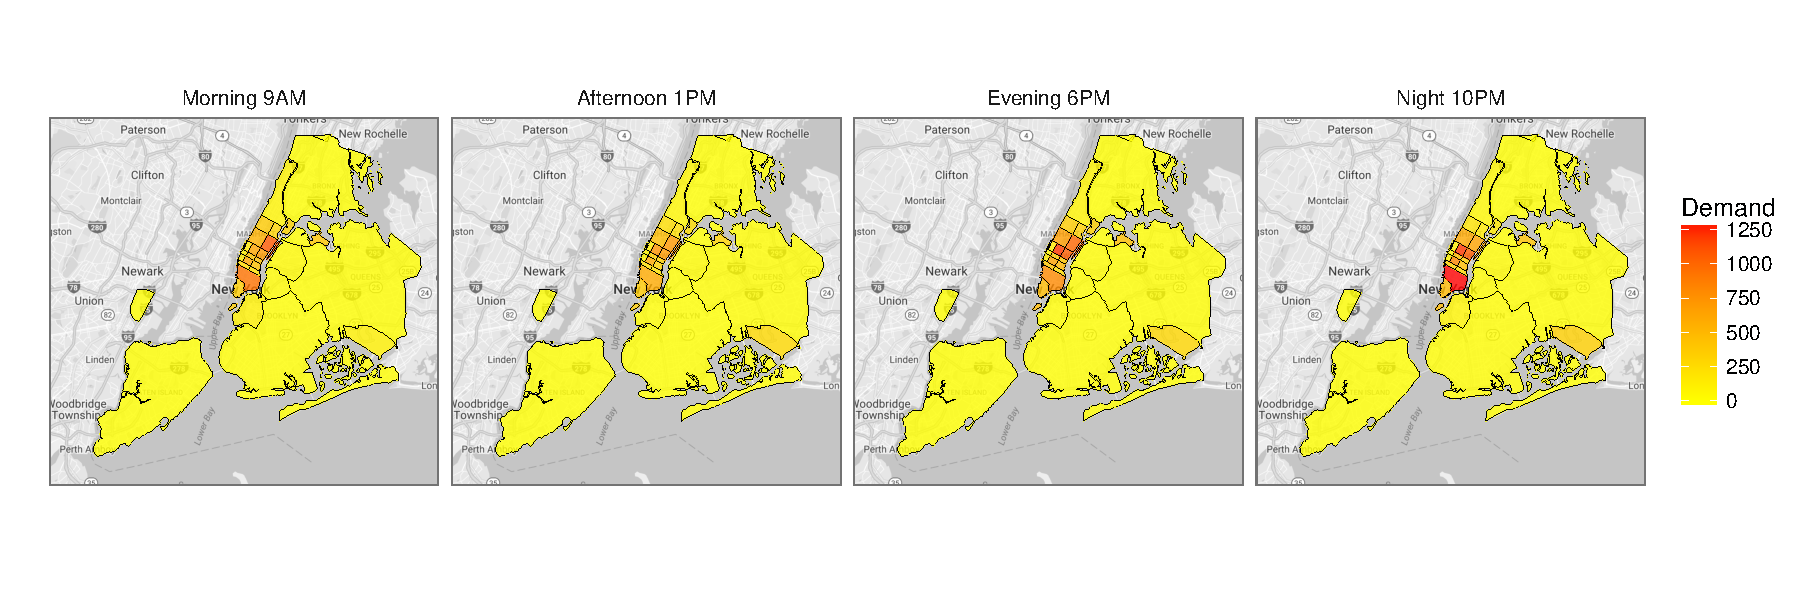
\includegraphics{figures/demand_heatmap.pdf}
	\caption{Demand across NYC zones.}
	\label{fig:demand_heatmap}
	%\fnote{Rides starting from each zone in NYC at different times of the day. Notably, inside Manhattan, the popular travel direction reverses from morning to evening, as expected.}
\end{figure}

Similarly, travel time matrix $\traveltimematrix^t$ and rewards matrix $\rewardsmatrix^t$ entries contain the average travel times and average rewards of traveling between two zones. Note that each entry of the {\rewardsmatrix} matrix represents net reward, calculated after taking into account the surge information, along with driver expenses and Uber's share of earnings.

Now, we describe the formation of the empirical transition matrix {\empiricaltransitionmatrix}. Every diagonal entry of the count matrix {\countmatrix} is zero, as there are no passenger rides within same zone. However, the empirical transition matrix {$\empiricaltransitionmatrix^t$} described in Section \ref{sec:problem_setup} assumes that the diagonal entries $f(i,i)$ denote the probabilities of a driver not finding a passenger in zone $i$ in the time-slice $t$. Hence, to form the empirical transition matrix, we first normalize the observed count matrix such that each of its rows sum up to 1 and call this matrix $\countmatrix^\prime$. In the following section, we describe the modifications to $\countmatrix^\prime$ to make it compliant with our definition.

\spara{Modeling successful passenger pickup}:
We use {\passengerarrivalrate} and {\driverarrivalrate} to denote the Poisson arrival rates of passengers and drivers in the time-slice $t$, within a zone $i$. Correspondingly, $N(\passengerarrivalrate)$ and $N(\driverarrivalrate)$ denote the number of passenger and driver arrivals in zone $i$ in one time unit. Assuming that passenger and driver arrivals are independent Poisson processes, the random variable $K = N(\passengerarrivalrate) - N(\driverarrivalrate)$ follows \textit{Skellam Distribution} as follows,
\begin{equation}
\Pr[K=k] = e^{-(\passengerarrivalrate + \driverarrivalrate)} \bigg(\frac{\passengerarrivalrate}{\driverarrivalrate}\bigg) I_k\big(2 \sqrt{\passengerarrivalrate \driverarrivalrate}\big)
\end{equation}
where $I_k(z)$ is the modified Bessel function of the first kind. We can depict the random variable $K$ as states of a {\markovchain}\footnote{Although, for simplicity, we assume the independence of the passenger and driver arrival processes, we can also accommodate correlated processes with slight modification.}.

% in Figure \ref{fig:skellam_markov_chain}.


% \begin{figure}
% \begin{center}
% \begin{tikzpicture}[->, >=stealth', auto, semithick, node distance=2cm]
% \tikzstyle{every state}=[fill=white,draw=black,thick,text=black,scale=0.65]
% \node[state]    (-inf)               {$\bf ...$};
% \node[state]    (-2)[right of=-inf]   {$\bf -2$};
% \node[state]    (-1)[right of=-2]   {$\bf -1$};
% \node[state]    (0)[right of=-1]   {$\bf 0$};
% \node[state]    (+1)[right of=0]   {$\bf 1$};
% \node[state]    (+2)[right of=+1]   {$\bf 2$};
% \node[state]    (+inf) [right of=+2] {$\bf ...$};
% \path
% (-inf)  edge[bend left]         node{$\passengerarrivalrate$}   (-2)
% (-2)    edge[bend left]         node{$\passengerarrivalrate$}   (-1)
%         edge[bend left,below]   node{$\driverarrivalrate$}       (-inf)
% (-1)    edge[bend left]         node{$\passengerarrivalrate$}   (0)
%         edge[bend left,below]   node{$\driverarrivalrate$}       (-2)
% (0)     edge[bend left]         node{$\passengerarrivalrate$}   (+1)
%         edge[bend left,below]   node{$\driverarrivalrate$}       (-1)
% (+1)    edge[bend left]         node{$\passengerarrivalrate$}   (+2)
%         edge[bend left,below]   node{$\driverarrivalrate$}       (0)
% (+2)     edge[bend left]        node{$\passengerarrivalrate$}   (+inf)
%         edge[bend left,below]   node{$\driverarrivalrate$}       (+1)
% (+inf)  edge[bend left,below]   node{$\driverarrivalrate$}       (+2);
% \end{tikzpicture}
% \caption{Markov Chain depiction of Skellam Distribution}
% \label{fig:skellam_markov_chain}
% \end{center}
% \end{figure}

Whenever the {\markovchain} is in a non-positive state, there are more drivers than passengers in a given zone. We assume the worst case scenario in which our driver of interest is at the last spot of a FIFO queue. Hence, for a state $k \leq 0$, the driver has to wait for $(|k| + 1)$ passenger arrivals in a unit time for a successful passenger pickup. The probability of a successful passenger pickup can be expressed as,
\begin{equation}
\Pr[N(\passengerarrivalrate) = |k| + 1] = \frac{\passengerarrivalrate^{\big(|k|+1\big)} e^{-\passengerarrivalrate}}{\big(|k| + 1\big)!}
\end{equation}
Thus, we can express a diagonal entry $f(i,i)$ of empirical transition matrix as follows,
\begin{equation}
f(i,i) = 1 - \sum_{k \leq 0} \Pr[K = k] \times \Pr[N(\passengerarrivalrate) \geq |k| + 1]
\end{equation}
To maintain the right stochasticity of {\empiricaltransitionmatrix}, every other entry $f(i,j)$ is calculated as,
\begin{equation}
f(i,j) = (1 - f(i,i)) \times c^\prime(i,j)
\end{equation}
The matrix {\empiricaltransitionmatrix}, built in this manner satisfies all our assumptions and can be used in the evaluation of strategies described in previous sections.

\begin{figure*}
	\centering
	\caption{Daily earnings with different strategies}
	\label{fig:daily_earnings}
	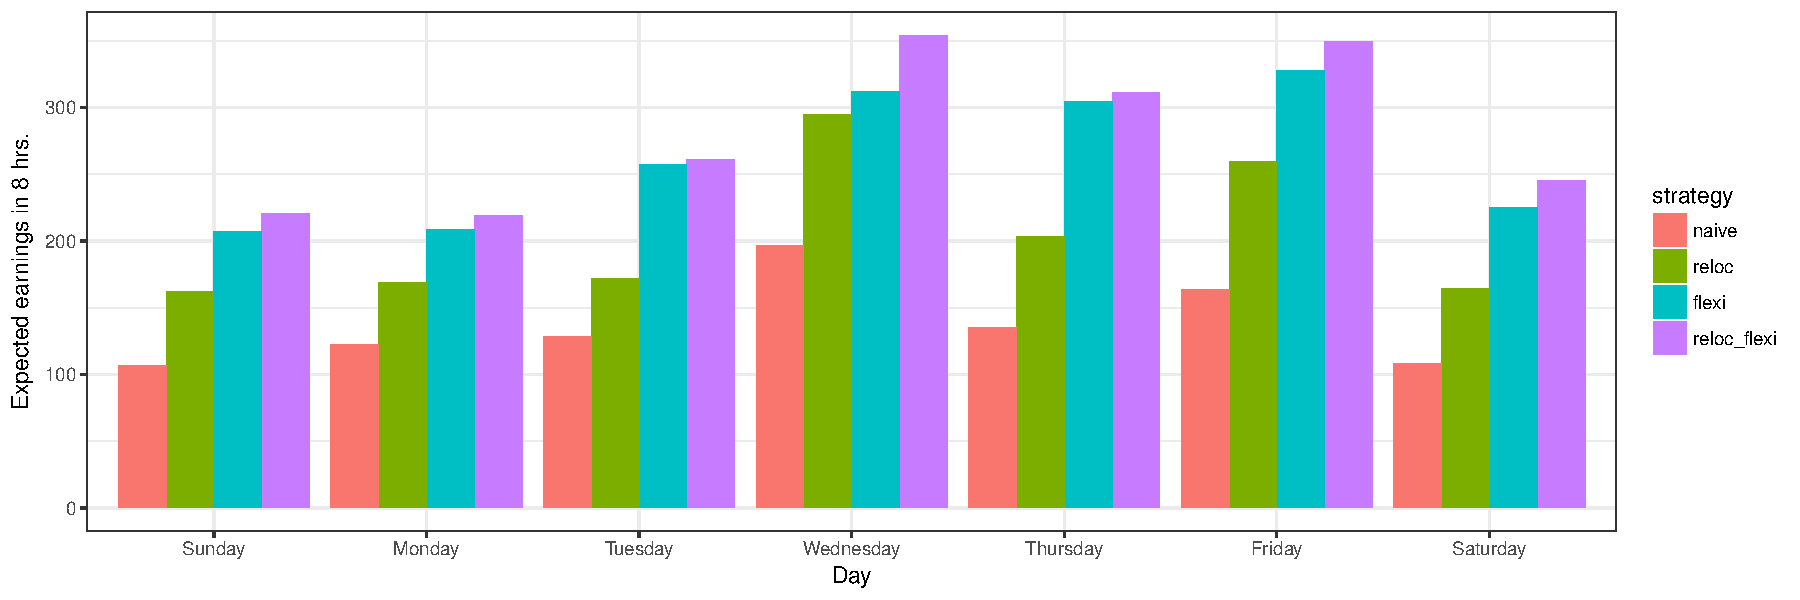
\includegraphics{figures/daily_earnings.pdf}
\end{figure*}

\subsection{Experiments}
In this section, we describe various experiments aimed at evaluating various aspects of the driver strategies formulated in Section \ref{sec:driver_strategies} using the experimental framework described in the previous section.

\spara{Comparison of strategies}: Here, we answer the question: \textit{what is the best driver strategy?} Intuitively, it is clear that {\relocationflexible} strategy is the best strategy as it takes advantage of spatial as well as temporal variations in the passenger demand across NYC. In order to verify this intuition, we compare driver earnings across different strategies. Drivers following the {\naive} and the {\relocation} strategies are assumed to drive from 9AM to 5PM, an 8 hour work day, while those following the {\flexible} or the {\relocationflexible} strategies drive for 8 hours each day with a flexible schedule.

Figure \ref{fig:daily_earnings} plots the solution to the {\originalproblem} for each of the strategies on different days of the week. For each of the day, We observe that driver earnings from {\relocationflexible} strategy are more than twice of those from {\naive}. The {\flexible} strategy always provides better earnings than even a {\relocation} strategy in 9 to 5 work schedule. Furthermore, we also observe that midweek earnings from all strategies exceed those on weekends.

\spara{Spatial dynamics of strategies}: Here, we explore the question - \textit{what are the benefits of the relocation action?} Figure \ref{fig:demand_heatmap} already shows the spatial variation in the demand across different NYC zones at different times of the day. Intuitively, this spatial variation can cause a disparity in the driver earnings based upon the zone of the driver. The {\relocation} strategy tries to reduce this disparity by allowing a driver to relocate while in a zone of low demand. To test our hypothesis, we calculate earnings from the {\naive} and the {\relocation} strategy from 8 hours of driving starting from every zone in the city, at different times of the day. We depict these earnings in form of a heatmap in Figure \ref{fig:earnings_heatmap}.

\begin{figure*}[hb]
	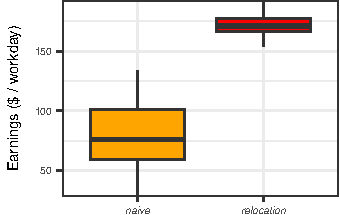
\includegraphics{figures/earnings_heatmap.pdf}
	\caption{Earnings across NYC zones with \textit{naive} and \textit{relocation} strategy.}
	\label{fig:earnings_heatmap}
\end{figure*}

We observe that, as expected, the variation in the {\naive} strategy earnings is substantial at all times of the day. Most notably, in the morning hours, drivers from zones surrounding Manhattan and those from near JFK airport earn considerably more than others. The {\relocation} strategy balances out this variation in earnings to some extent, while consistently outperforming the {\naive} strategy across all zones.

\spara{Temporal dynamics of strategies}: It is obvious from Figure \ref{fig:daily_earnings} that both of the flexible schedule strategies outperform their fixed schedule counterparts. So, we explore the question \textit{what is the best time of the day to drive in order to maximize earnings?} As the choice of the {\gohome} action depends on multiple factors such as the location of the driver, the demand across the city, the budget left, etc., we visualize preferred driving hours using 1000 simulated drivers. Each driver has a randomly assigned home zone. At every step throughout the day, simulated drivers follow actions recommended by the contingency plans developed while solving the {\originalproblem} for {\flexible} and {\relocationflexible} strategies.

\begin{figure}[H]
	\centering
	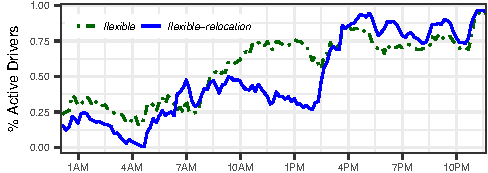
\includegraphics[scale=0.75]{figures/simulated_schedules.pdf}
	\caption{Active drivers with {\flexible} and {\relocationflexible}
	strategies at different times of the day.}
	\label{fig:simulated_schedules}
\end{figure}

We observe that drivers of both {\flexible} and {\relocationflexible} strategies are active in large percentages after 7PM in the evening. However, over 50\% of the drivers following the {\flexible} strategy are active throughout the day after 8AM in the morning. In stark contrast with them, drivers following the {\relocationflexible} strategy are active in overwhelming percentages during peak hours of the day, from 6AM to 10AM in the morning, and post 7PM in the evening. This makes us conclude that {\relocate} action is more effective during the peak hours, thereby prompting higher percentages of {\relocationflexible} drivers to be active in those hours.

\spara{Preferred relocation zones}:
Simulated drivers also allow us to compare the {\relocate} actions between drivers following {\relocation} strategy and those following {\relocationflexible} strategy. The endzones for relocate actions of drivers are shown in Figure \ref{fig:relocation_endzones}. We observe a contrast between the preferred relocation zones for drivers of either strategies. Drivers following the {\relocation} strategy predominantly relocate themselves to zones `3A', `3C', `4A' zones near the West Village neighborhood and zones `7B' and `8' near the LaGuardia Airport, while those following the {\relocationflexible} strategy relocate themselves to zone `1' comprising of the Financial District and zones `5A', `5B' and `6B' near the Upper East side of New York City.

\begin{figure*}
	\centering
	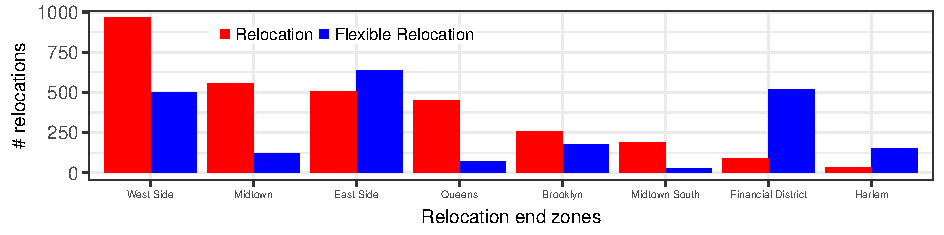
\includegraphics{figures/relocation_endzones.pdf}
	\caption{Contrast between preferred relocation endzones for drivers with 
	{\relocation} and {\relocationflexible} strategies}
	\label{fig:relocation_endzones}
\end{figure*}

\spara{Surge Chasing}:
Now that we have an understanding about the various driver strategies, we turn our attention to surge pricing. Surge pricing is a controversial feature of the Uber platform. According to Uber, it encourages drivers to start driving during the peak hours in order to efficiently meet demand with supply, albeit at a higher cost to passenger, in turn leading to higher driver earnings. In fact, Uber prominently displays to drivers on their Partner App, the information regarding surge multiplier in different geographical neighborhoods in form of a heatmap. However, as the Uber's surge pricing algorithm is proprietary, it is unclear whether drivers should relocate themselves to surging areas consistently in order to maximize their earnings. Using our information about surge multipliers, we are in a position to answer the question-- \textit{Should drivers engage in surge chasing?}
\begin{figure}[H]
	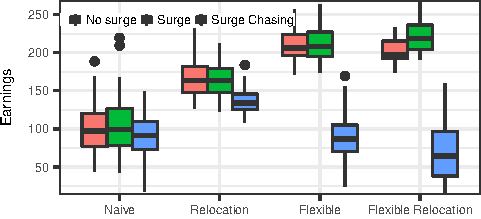
\includegraphics{figures/simulated_earnings.pdf}
	\caption{Simulated earnings for drivers across different strategies.}
	\label{fig:simulated_earnings}
\end{figure}
In order to do so, we evaluate earnings of simulated drivers in three scenarios viz., `no surge' - where we disable the surge multiplier, `surge' - where surge multiplier is accounted for while calculating earnings, and `surge chasing' wherein surge multiplier is enabled and a driver `chases surge' i.e, a driver located in a non-surging zone always relocates to the zone with highest surge multiplier. The earnings of the simulated drivers in these scenarios are shown in Fig. {\ref{fig:simulated_earnings}}. We observe that `chasing surge' in {\naive} strategy on an average yields slightly less earnings than even the situation when surge multiplier is disabled. Interestingly, chasing surge is even more ill-advised if the driver follows a flexible schedule strategy, and it can lead to huge losses.

\subsection{Effect of uncertainty} 

All the experiments described in previous section indicate that our strategies always outperform a {\naive} strategy most prevalent among the drivers. However, it is worth noting that our strategies are evaluated based on historical data. Consequently, such strategies can be highly sensitive to changes in the underlying data, in form of perturbed transition matrices. We can recommend our strategies to drivers only if they outperform the {\naive} strategy in presence of such perturbations. Hence, using the framework developed in Section \ref{sec:sensitivity}, we solve the {\robustproblem} problem for each of the four strategies for increasing levels of uncertainty in the transition matrices.

Figure \ref{fig:uncertainty_evolution} shows the results of increasing uncertainty on the earnings of drivers following each of the four strategies. Not only are the {\relocation}, {\flexible} and {\relocationflexible} strategies more tolerant to uncertainty in transition matrices, but they outperform the {\naive} strategy at 0\% uncertainty, while themselves at with 99\% uncertainty. This provides evidence regarding the robustness of such strategies.

\begin{figure}[H]
	\centering
	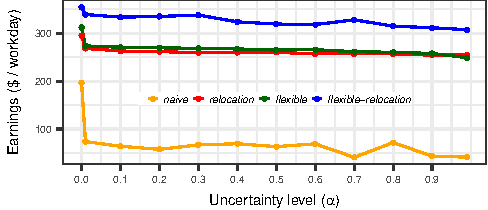
\includegraphics{figures/uncertainty_evolution.pdf}
	\caption{Sensitivity to uncertainty in parameters.}
	\label{fig:uncertainty_evolution}
\end{figure}

\begin{figure*}[hb]
	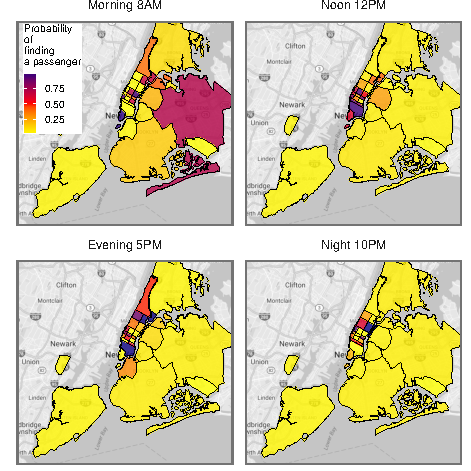
\includegraphics{figures/successful_heatmap.pdf}
	\caption{Probability of finding a passenger in 1 time unit across NYC zones at different times of the day.}
	\label{fig:successful_heatmap}
\end{figure*}

\begin{figure*}[hb]
	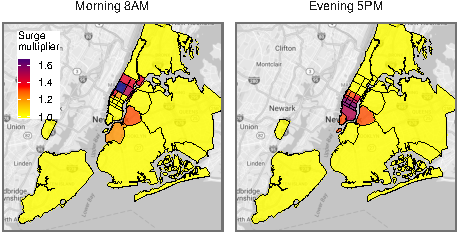
\includegraphics{figures/surge_heatmap.pdf}
	\caption{Active surge multiplier across NYC zones at different times of the day.}
	\label{fig:surge_heatmap}
\end{figure*}

% \subsection{\textsc{RewardsMatrix}}

% The data gathered in the previous section gives us a matrix of driver earnings, \matr{E}, from passengers while traveling between any two zones in the city. We also get a costs matrix, \matr{C}, whose each entry, $c(i,j) \leq 0$, denotes the sundry expenses of traveling from zone $i$ to zone $j$, dependent on distance and traffic at the given time. The travel costs can result in negative net rewards in the {\gohome} and {\relocate} actions, violating the assumption from Section \ref{sec:problem_setup} that $r(i,j) \geq 0$. In this section, we describe the construction of \textsc{RewardsMatrix}, {\rewardsmatrix}, corresponding to each driver action compliant with our assumptions.

% \subsubsection{\textsc{Modifying the CostsMatrix}}
% If $min\_cost$ is the minimum entry in the matrix \matr{C}, each entry of the modified costs matrix, \matr{C'} is calculated as,
% \begin{equation}
% c'(i,j) = c(i,j) - min\_cost
% \end{equation}
% As a result of the above modification, $\forall i,j : c'(i,j) \geq 0$.

% \subsubsection{\textsc{RewardsMatrix}}
% In order to be compliant with the assumption in Section \ref{sec:problem_setup}, we define two kinds of \textsc{RewardsMatrix}, one for the action {\getpassenger} and another for the actions {\gohome} and {\relocate}.

% \begin{itemize}
% 	\item For the {\getpassenger} action, we define the rewards matrix as,
% 	\begin{equation}
% 		r(i,j) = e(i,j) + c'(i,j) 
% 	\end{equation}
% 	\item For the {\gohome} and {\relocate} actions, the rewards matrix is same as the modified costs matrix.
% 	\begin{equation}
% 		r(i,j) = c'(i,j)
% 	\end{equation}
% \end{itemize}
% In both cases, we set the diagonal entries of the matrix to zero i.e., $\forall i: r(i,i) = 0$.

% It should be noted that this modification does not affect the optimal action choice in any strategy. It merely ensures that the input vectors to the Bisection Algorithm from Section \ref{sec:sensitivity} are always non-negative vectors. Furthermore, while calculating the actual {\totalexpectedearnings} of a driver, we can backtrack these modifications.

% \subsection{\textsc{Comparing robust and nominal strategies}}
% In this section, we compare various strategies. When we choose, $\beta = \betamax$, there is no uncertainty, and we get solution computed via the classical Bellman recursion; referred to as nominal strategy. The robust strategy corresponds to solving the MDP with varying values of $\beta$.

% \subsection{\textsc{Effect of Inaccuracy is uncertainty level}}
% The previous section assumes that, in the robust case, we are able to estimate exactly the precise value of the uncertainty level. In practice, the parameter $\beta$ also has to be estimated. In this section, we study the sensitivity of the robust approach with respect to inaccuracies in the uncertainty parameter $\beta$.